% !TEX root = ../main.tex

\chapter{Appendix}
\label{ch:appendix}

\section{Hardware}
\label{sec:appendix-hardware}

\placeholderfigure{
  \textbf{Content.} The complete schematic, one landscape page per sheet. \textbf{How to obtain.} \code{kicad-cli sch export pdf hardware/ExpressionController.kicad\_sch}, included with \code{\textbackslash includepdf} (package \code{pdfpages}, already loaded).
}

\begin{figure}[htbp]
  \centering
  \begin{subfigure}[b]{0.49\linewidth}
    \centering
    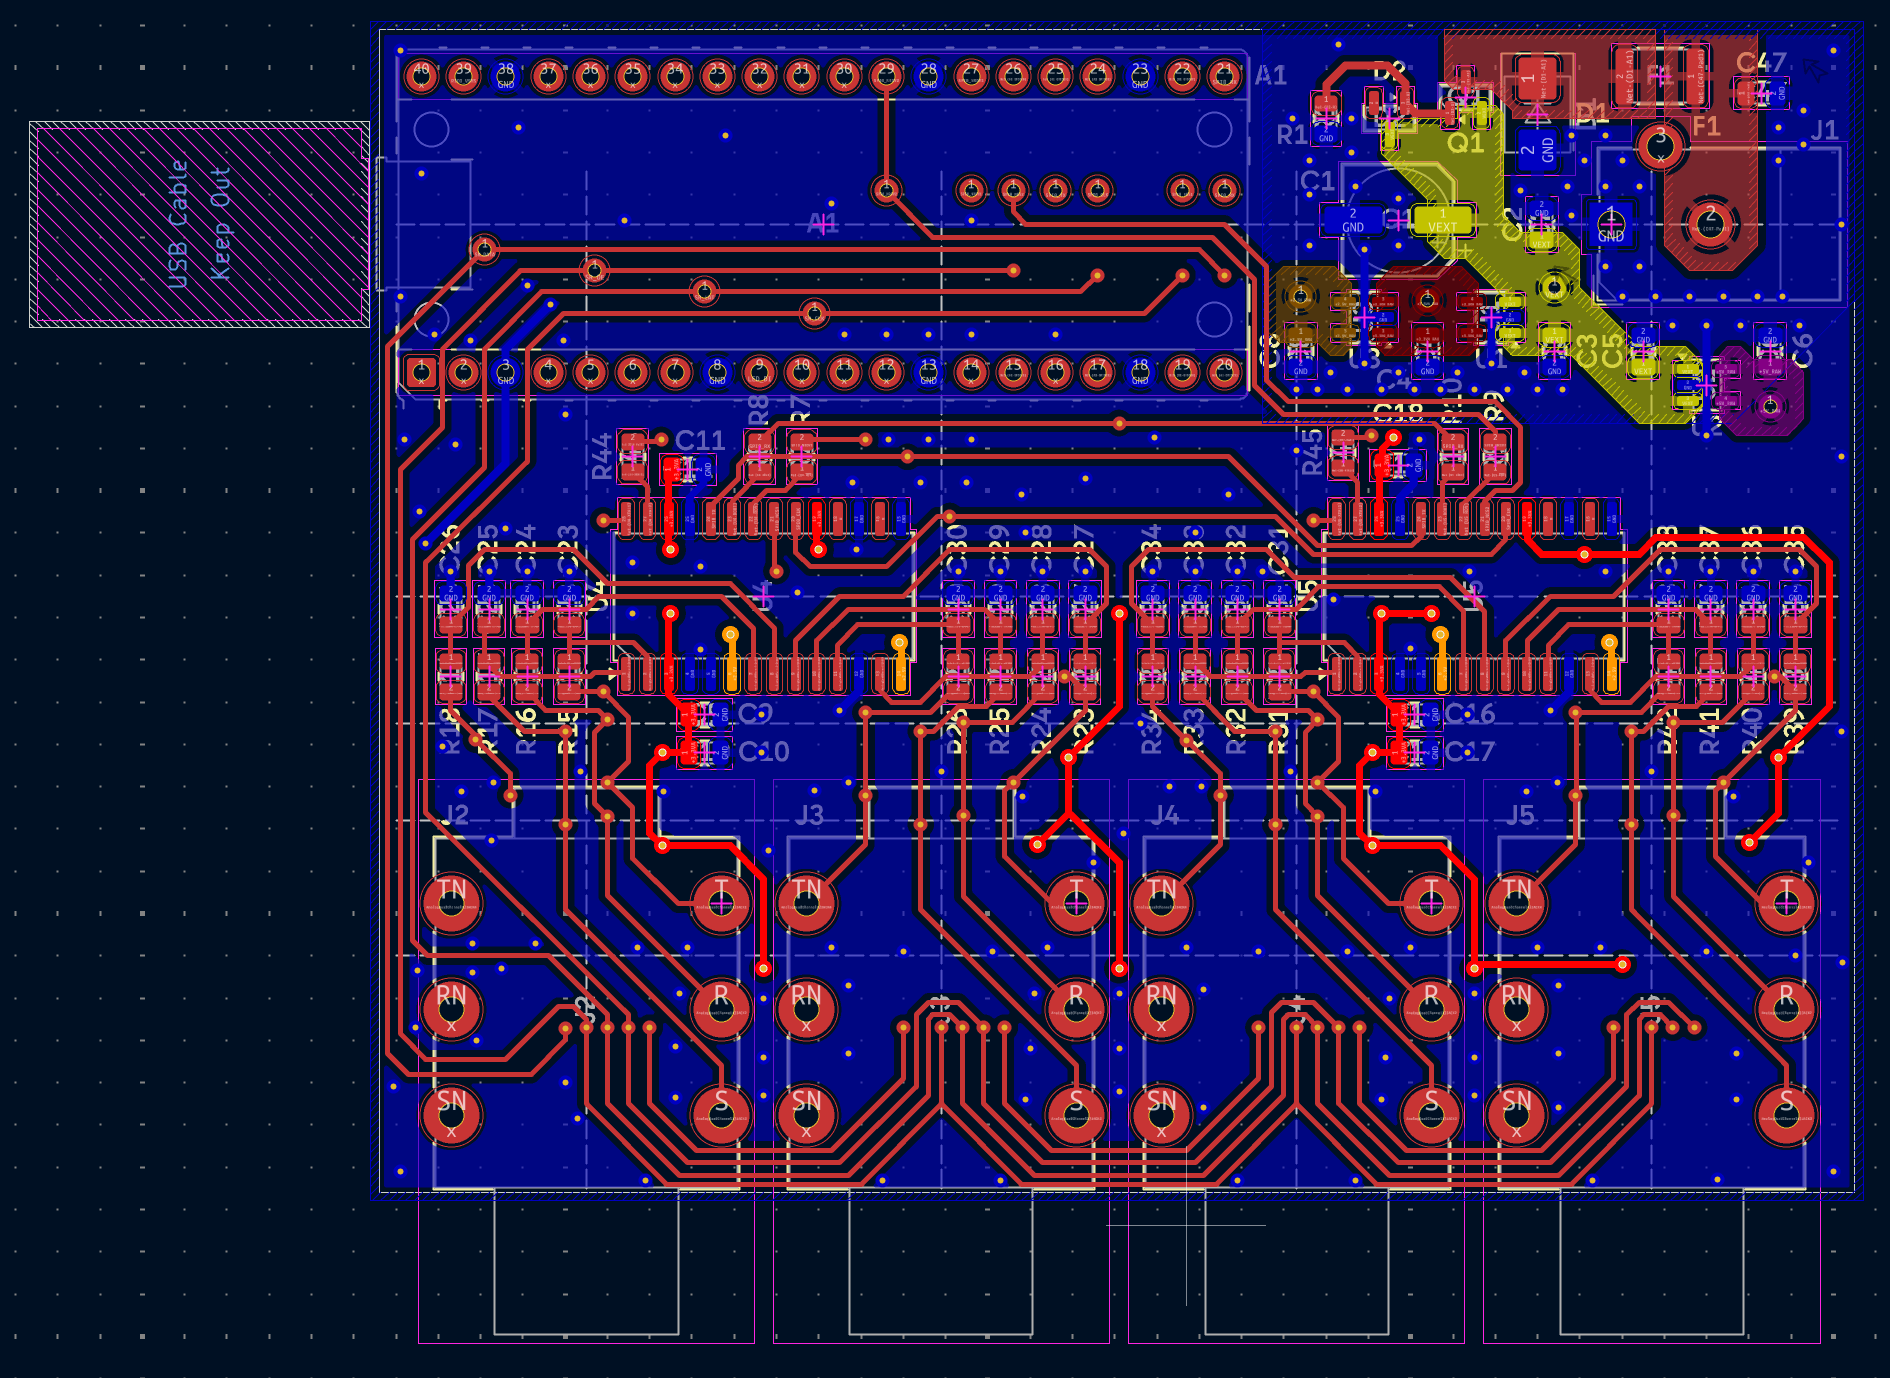
\includegraphics[width=\linewidth]{04-implementation/figures/pcb-layout}
    \caption{Layout}
    \label{fig:pcb-layout}
  \end{subfigure}%
  \hfill%
  \begin{subfigure}[b]{0.49\linewidth}
    \centering
    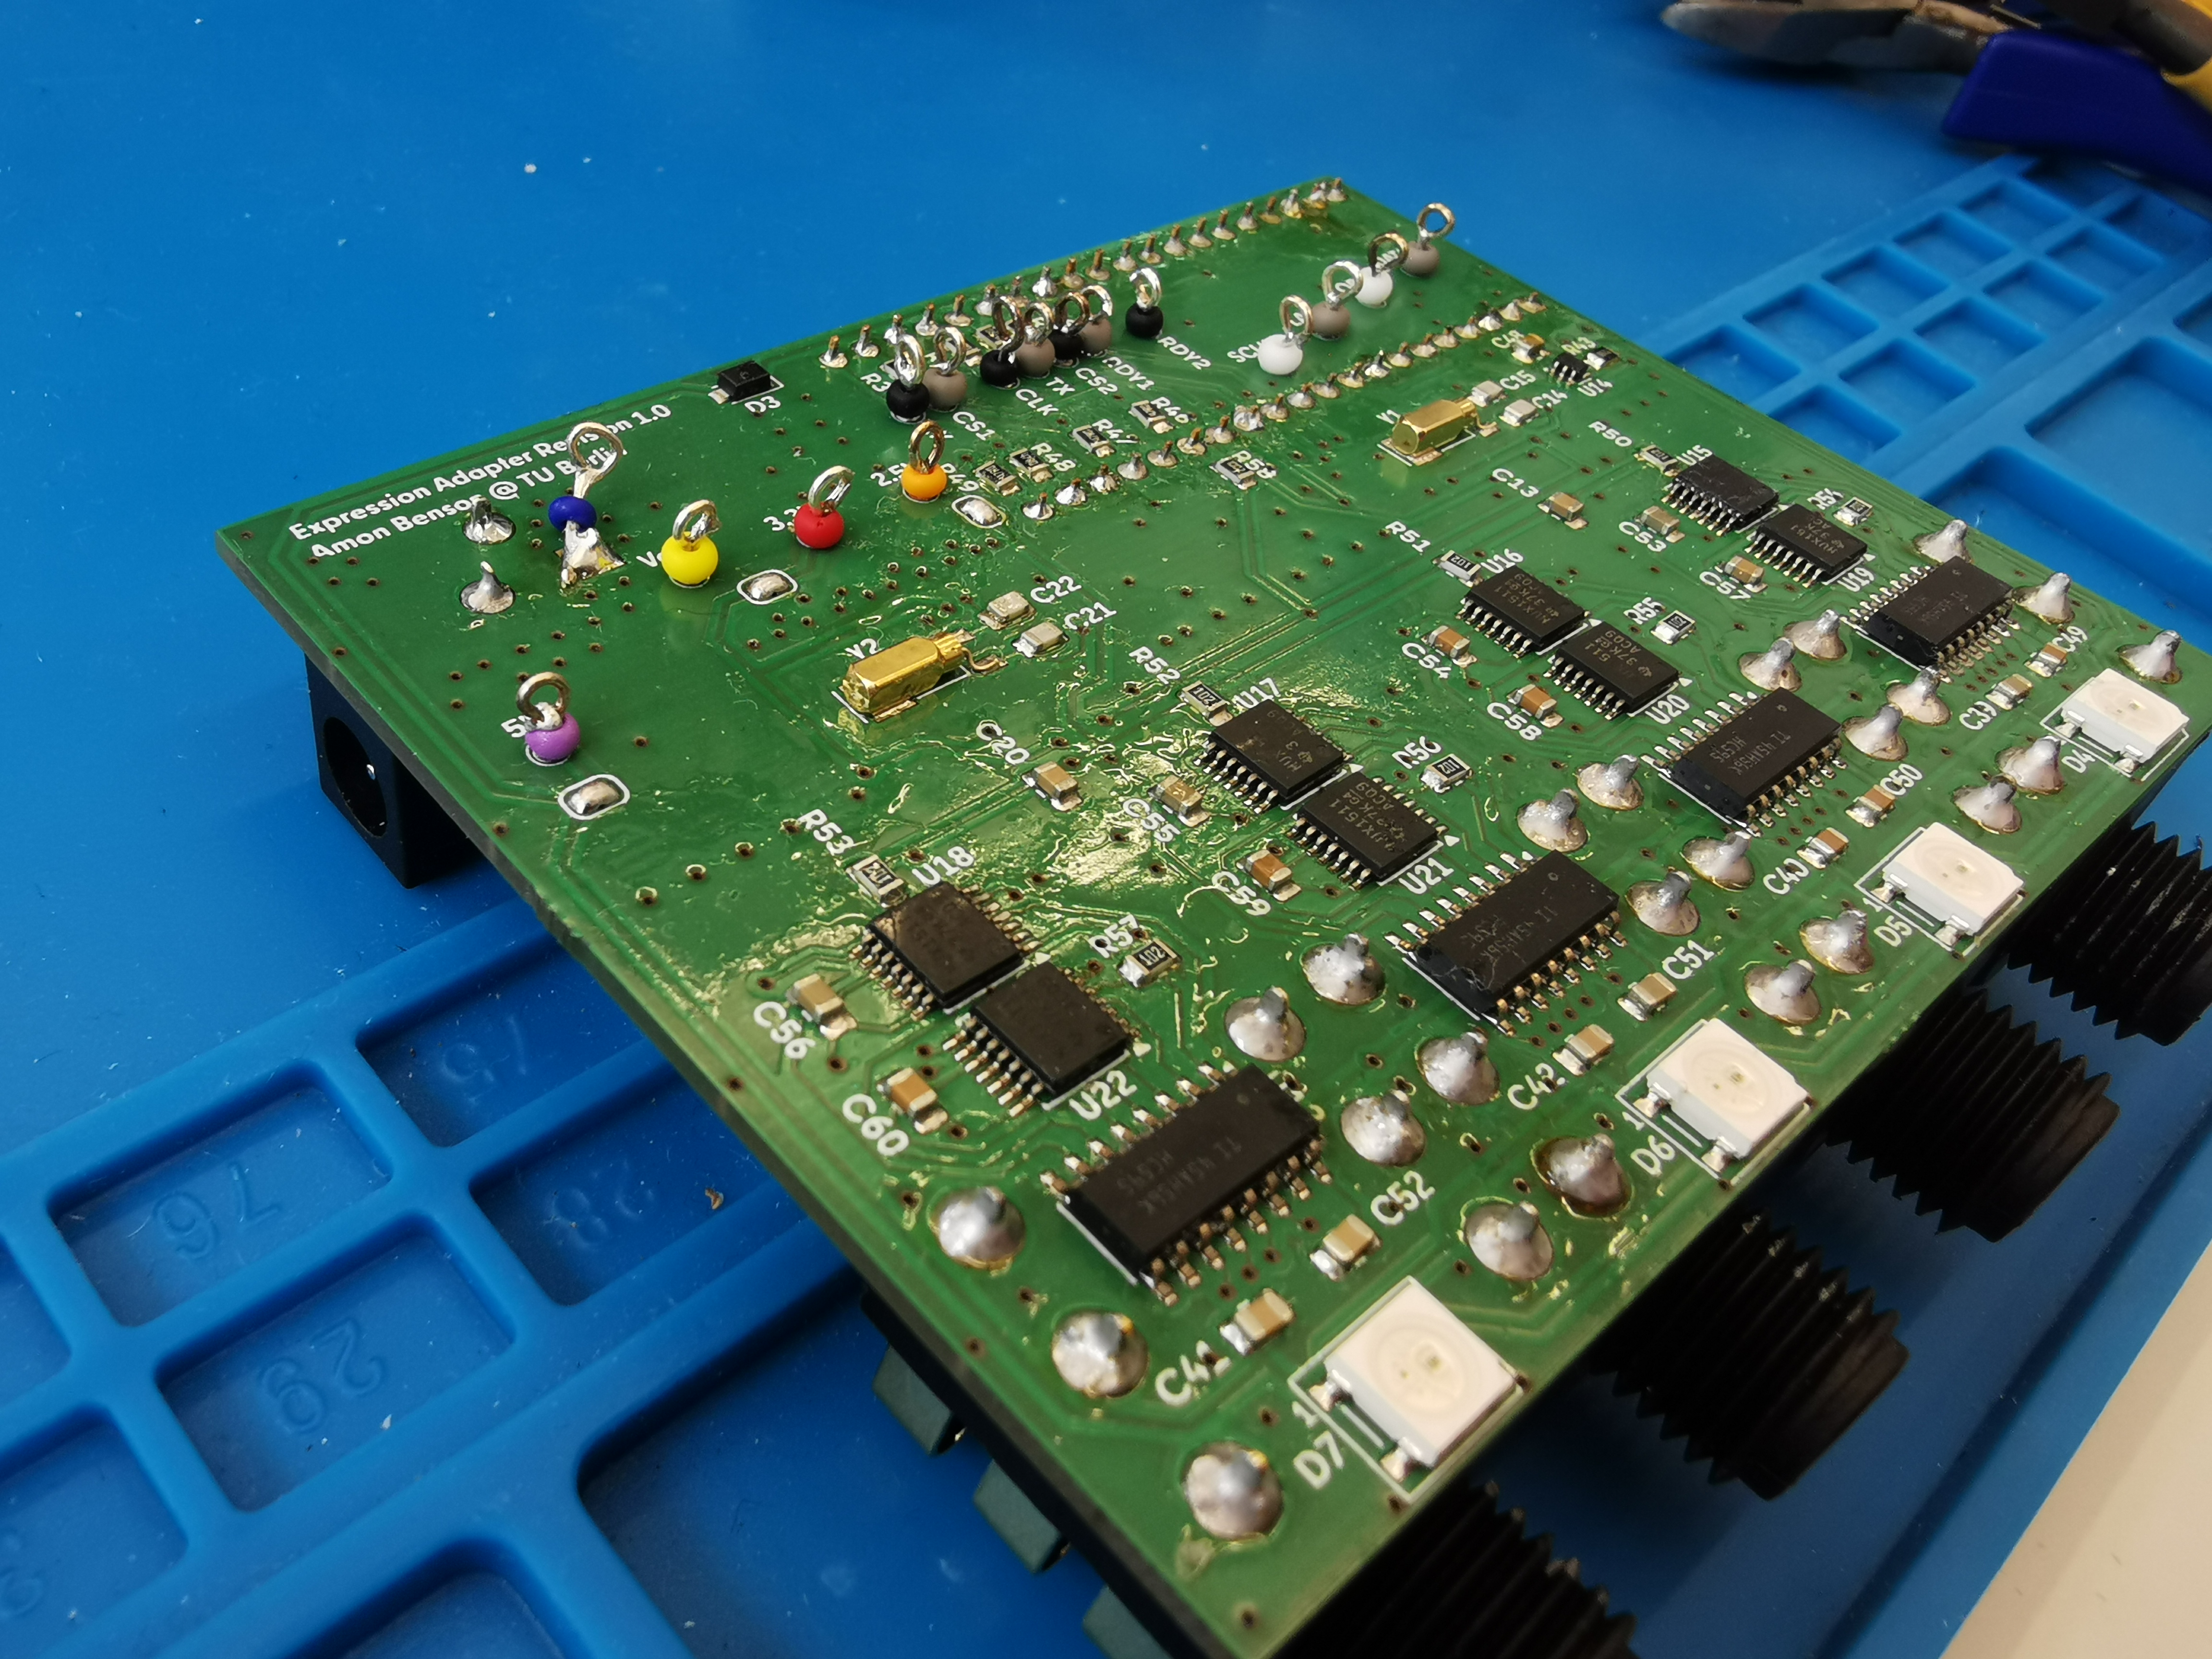
\includegraphics[width=\linewidth]{04-implementation/figures/assembly-complete}
    \caption{Assembled Board}
    \label{fig:assembly-complete}
  \end{subfigure}
  \titledcaption{PCB}{\scaffoldinline{Two-layer board, \qtyproduct{88.65 x 69.85}{\milli\metre}, manufactured by Aisler; name the regions (jacks, channel blocks, ADCs, microcontroller, power) and the color-coded test points.}}
  \label{fig:pcb}
\end{figure}

\section{Firmware}
\label{sec:appendix-firmware}

\begin{figure}[htbp]
  \centering
  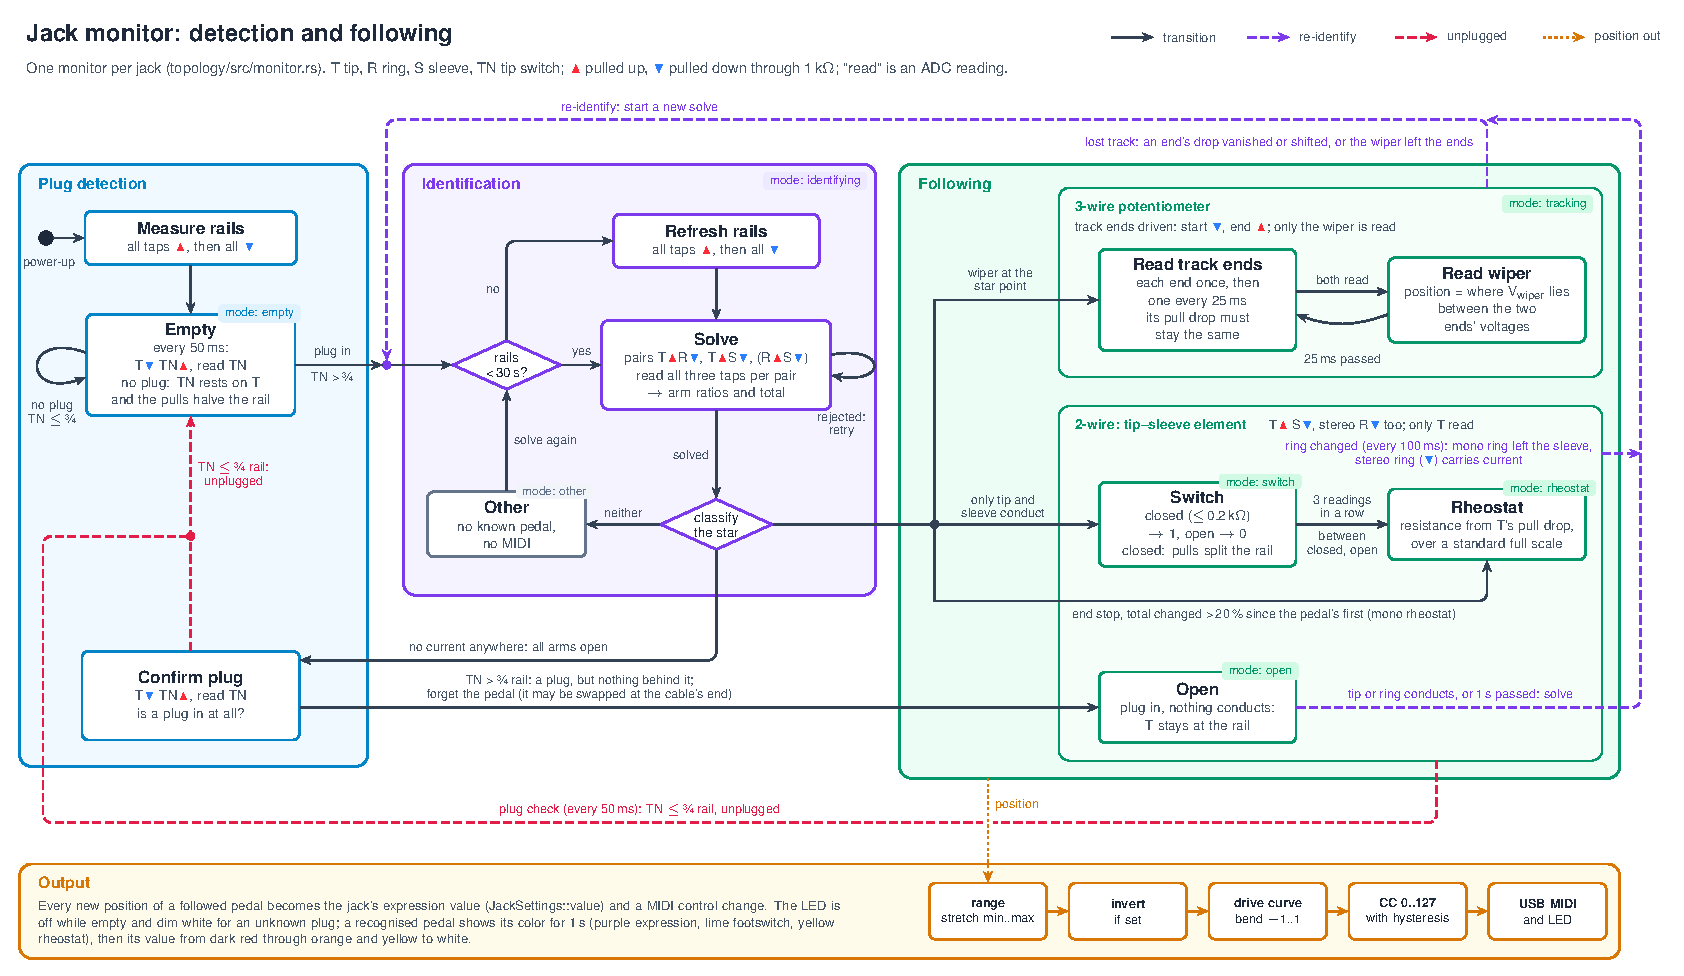
\includegraphics[width=\linewidth]{04-implementation/figures/jack-monitor-states}
  \titledcaption{Jack Monitor State Machine}{\scaffoldinline{Three groups (plug detection, identification, following), the mode of each state, the drive symbols, the two return corridors and the output strip. Source: \code{docs/diagrams/jack-monitor-states.tex}.}}
  \label{fig:jack-monitor-states}
\end{figure}

\begin{table}[htbp]
  \centering
  \footnotesize
  \titledcaption{Solver and Monitor Constants}{\scaffoldinline{Relative values refer to the total resistance; $\sigma$ is the noise of the checked quantity, derived from $\sigma_V = \qty{0.5}{\milli\volt}$. Sources: \code{SolverConfig::from\_voltage\_noise}, \code{MonitorConfig::new}.}}
  \label{tab:constants}
  \begin{tabular}{@{}ll@{\hspace{2em}}ll@{}}
    \toprule
    \textbf{Solver} & & \textbf{Monitor} & \\
    \midrule
    Pair conducts & $I > 3\sigma$ & Plug check & every \qty{50}{\milli\second} \\
    High and low current agree & $5\sigma$ or \qty{10}{\percent} & Track-end check & every \qty{25}{\milli\second} \\
    Pair totals agree & $4\sigma$ or \qty{10}{\percent} & Ring check & every \qty{100}{\milli\second} \\
    Short & pair $<\qty{50}{\ohm}$ & Rail refresh & after \qty{30}{\second} \\
    Ratio defined & span $> 10\,\sigma_V$ & Largest wiper arm & \qty{25}{\percent} \\
    Third pair & conditioning $< 0.5$ & End stop & \qty{2}{\percent} \\
    & & Track-end drop & \qty{3}{\percent} or $6\sigma$ (first: \qty{25}{\percent}) \\
    & & Closed switch & $\leq \qty{0.2}{\kilo\ohm}$ \\
    & & Rheostat & 3 readings between open and closed \\
    \bottomrule
  \end{tabular}
\end{table}

\section{Measurements}
\label{sec:appendix-measurements}

\begin{table}[htbp]
  \centering
  \footnotesize
  \titledcaption{Voltage Span and Pull Drop}{\scaffoldinline{Voltage across the pedal and drop across one pull resistor, \qty{2.5}{\volt} rail; \qty{1}{\kilo\ohm} is fitted.}}
  \label{tab:pull-resistance}
  \begin{tabular}{@{}l *{3}{c}@{}}
    \toprule
    \textbf{Pull resistance} & \textbf{\qty{10}{\kilo\ohm} pedal} & \textbf{\qty{100}{\kilo\ohm} pedal} & \textbf{\qty{500}{\kilo\ohm} pedal} \\
    \midrule
    \qty{1}{\kilo\ohm} & \qty{2.08}{\volt} / \qty{208}{\milli\volt} & \qty{2.45}{\volt} / \qty{24}{\milli\volt} & \qty{2.49}{\volt} / \qty{5}{\milli\volt} \\
    \qty{2.2}{\kilo\ohm} & \qty{1.74}{\volt} / \qty{382}{\milli\volt} & \qty{2.40}{\volt} / \qty{53}{\milli\volt} & \qty{2.48}{\volt} / \qty{11}{\milli\volt} \\
    \qty{4.7}{\kilo\ohm} & \qty{1.29}{\volt} / \qty{606}{\milli\volt} & \qty{2.29}{\volt} / \qty{107}{\milli\volt} & \qty{2.45}{\volt} / \qty{23}{\milli\volt} \\
    \qty{10}{\kilo\ohm} & \qty{0.83}{\volt} / \qty{833}{\milli\volt} & \qty{2.08}{\volt} / \qty{208}{\milli\volt} & \qty{2.45}{\volt} / \qty{49}{\milli\volt} \\
    \bottomrule
  \end{tabular}
\end{table}

\begin{table}[htbp]
  \centering
  \footnotesize
  \titledcaption{ADC Characterization}{\scaffoldinline{EV-30 in jack~1 held still, tip as wiper, ring high, sleeve low, calibrated at every rate; a reading includes the channel change; one MIDI step is \num{7874} ppm.}}
  \label{tab:adc-characterization}
  \begin{tabular}{@{}rrrrrr@{}}
    \toprule
    \textbf{Rate (\unit{\hertz})} & \textbf{Filter word} & \textbf{Reading (\unit{\milli\second})} & \textbf{Noise (\unit{\milli\volt})} & \textbf{Step (\unit{\milli\volt})} & \textbf{Position (ppm)} \\
    \midrule
    1365 & 3 & 2.89 & 1.93 & 3.88 & 887 \\
    1024 & 4 & 3.63 & 0.80 & 0.41 & 374 \\
    819 & 5 & 4.36 & 0.39 & 0.21 & 203 \\
    682 & 6 & 5.09 & 0.40 & 0.12 & 184 \\
    315 & 13 & 10.22 & 0.11 & 0.012 & 62 \\
    \bottomrule
  \end{tabular}
\end{table}

\begin{table}[htbp]
  \centering
  \footnotesize
  \titledcaption{ADC Noise on the Empty Board}{\scaffoldinline{\qty{315}{\hertz}, \qty{30}{\second} per drive state, ranges over both ADCs.}}
  \label{tab:adc-noise}
  \begin{tabular}{@{}llll@{}}
    \toprule
    \textbf{Input} & \textbf{Mean} & \textbf{Noise ($\sigma$)} & \textbf{Drift in \qty{30}{\second}} \\
    \midrule
    Contacts pulled low & \qty{+1.3}{\milli\volt} / \qty{+1.5}{\milli\volt} & 15 to \qty{23}{\micro\volt} & $\leq \qty{0.04}{\milli\volt}$ \\
    Contacts pulled high & \qtyrange{2.4998}{2.5001}{\volt} & 50 to \qty{60}{\micro\volt} & $\leq \qty{0.16}{\milli\volt}$ \\
    Grounded input AIN6 & \qty{+1.3}{\milli\volt} / \qty{+1.5}{\milli\volt} & 15 to \qty{21}{\micro\volt} & none \\
    Reference input AIN10 & \qtyrange{2.4999}{2.5000}{\volt} & 55 to \qty{85}{\micro\volt} & $\leq \qty{0.17}{\milli\volt}$ \\
    \bottomrule
  \end{tabular}
\end{table}

\begin{table}[htbp]
  \centering
  \footnotesize
  \titledcaption{Plug-In and Unplug Timing}{\scaffoldinline{Milliseconds after the tip switch changed; following starts one pair length (\qty{14.6}{\milli\second}) after the last latch.}}
  \label{tab:plug-in}
  \begin{tabular}{@{}lrrr@{}}
    \toprule
    \textbf{Run} & \textbf{Plug noticed} & \textbf{Last latch} & \textbf{Following / empty} \\
    \midrule
    Plug-in 1 (not fully seated, first pair repeated) & 4.9 & 50.9 & $\approx$ 65 \\
    Plug-in 2 & 47.3 & 80.7 & $\approx$ 95 \\
    Plug-in 3 & 45.6 & 75.0 & $\approx$ 90 \\
    Plug-in 4 & 17.6 & 51.1 & $\approx$ 66 \\
    Plug-in 5 & 35.5 & 68.9 & $\approx$ 84 \\
    Plug-in, rails older than \qty{30}{\second} & 49.4 & 292.7 & $\approx$ 300 \\
    Unplug 1 / 2 / 3 & 1.8 / $\approx$5 / 26.7 & -- & 260 / 391 / 330 \\
    \bottomrule
  \end{tabular}
\end{table}

\begin{figure}[htbp]
  \centering
  \begin{subfigure}[b]{0.49\linewidth}
    \centering
    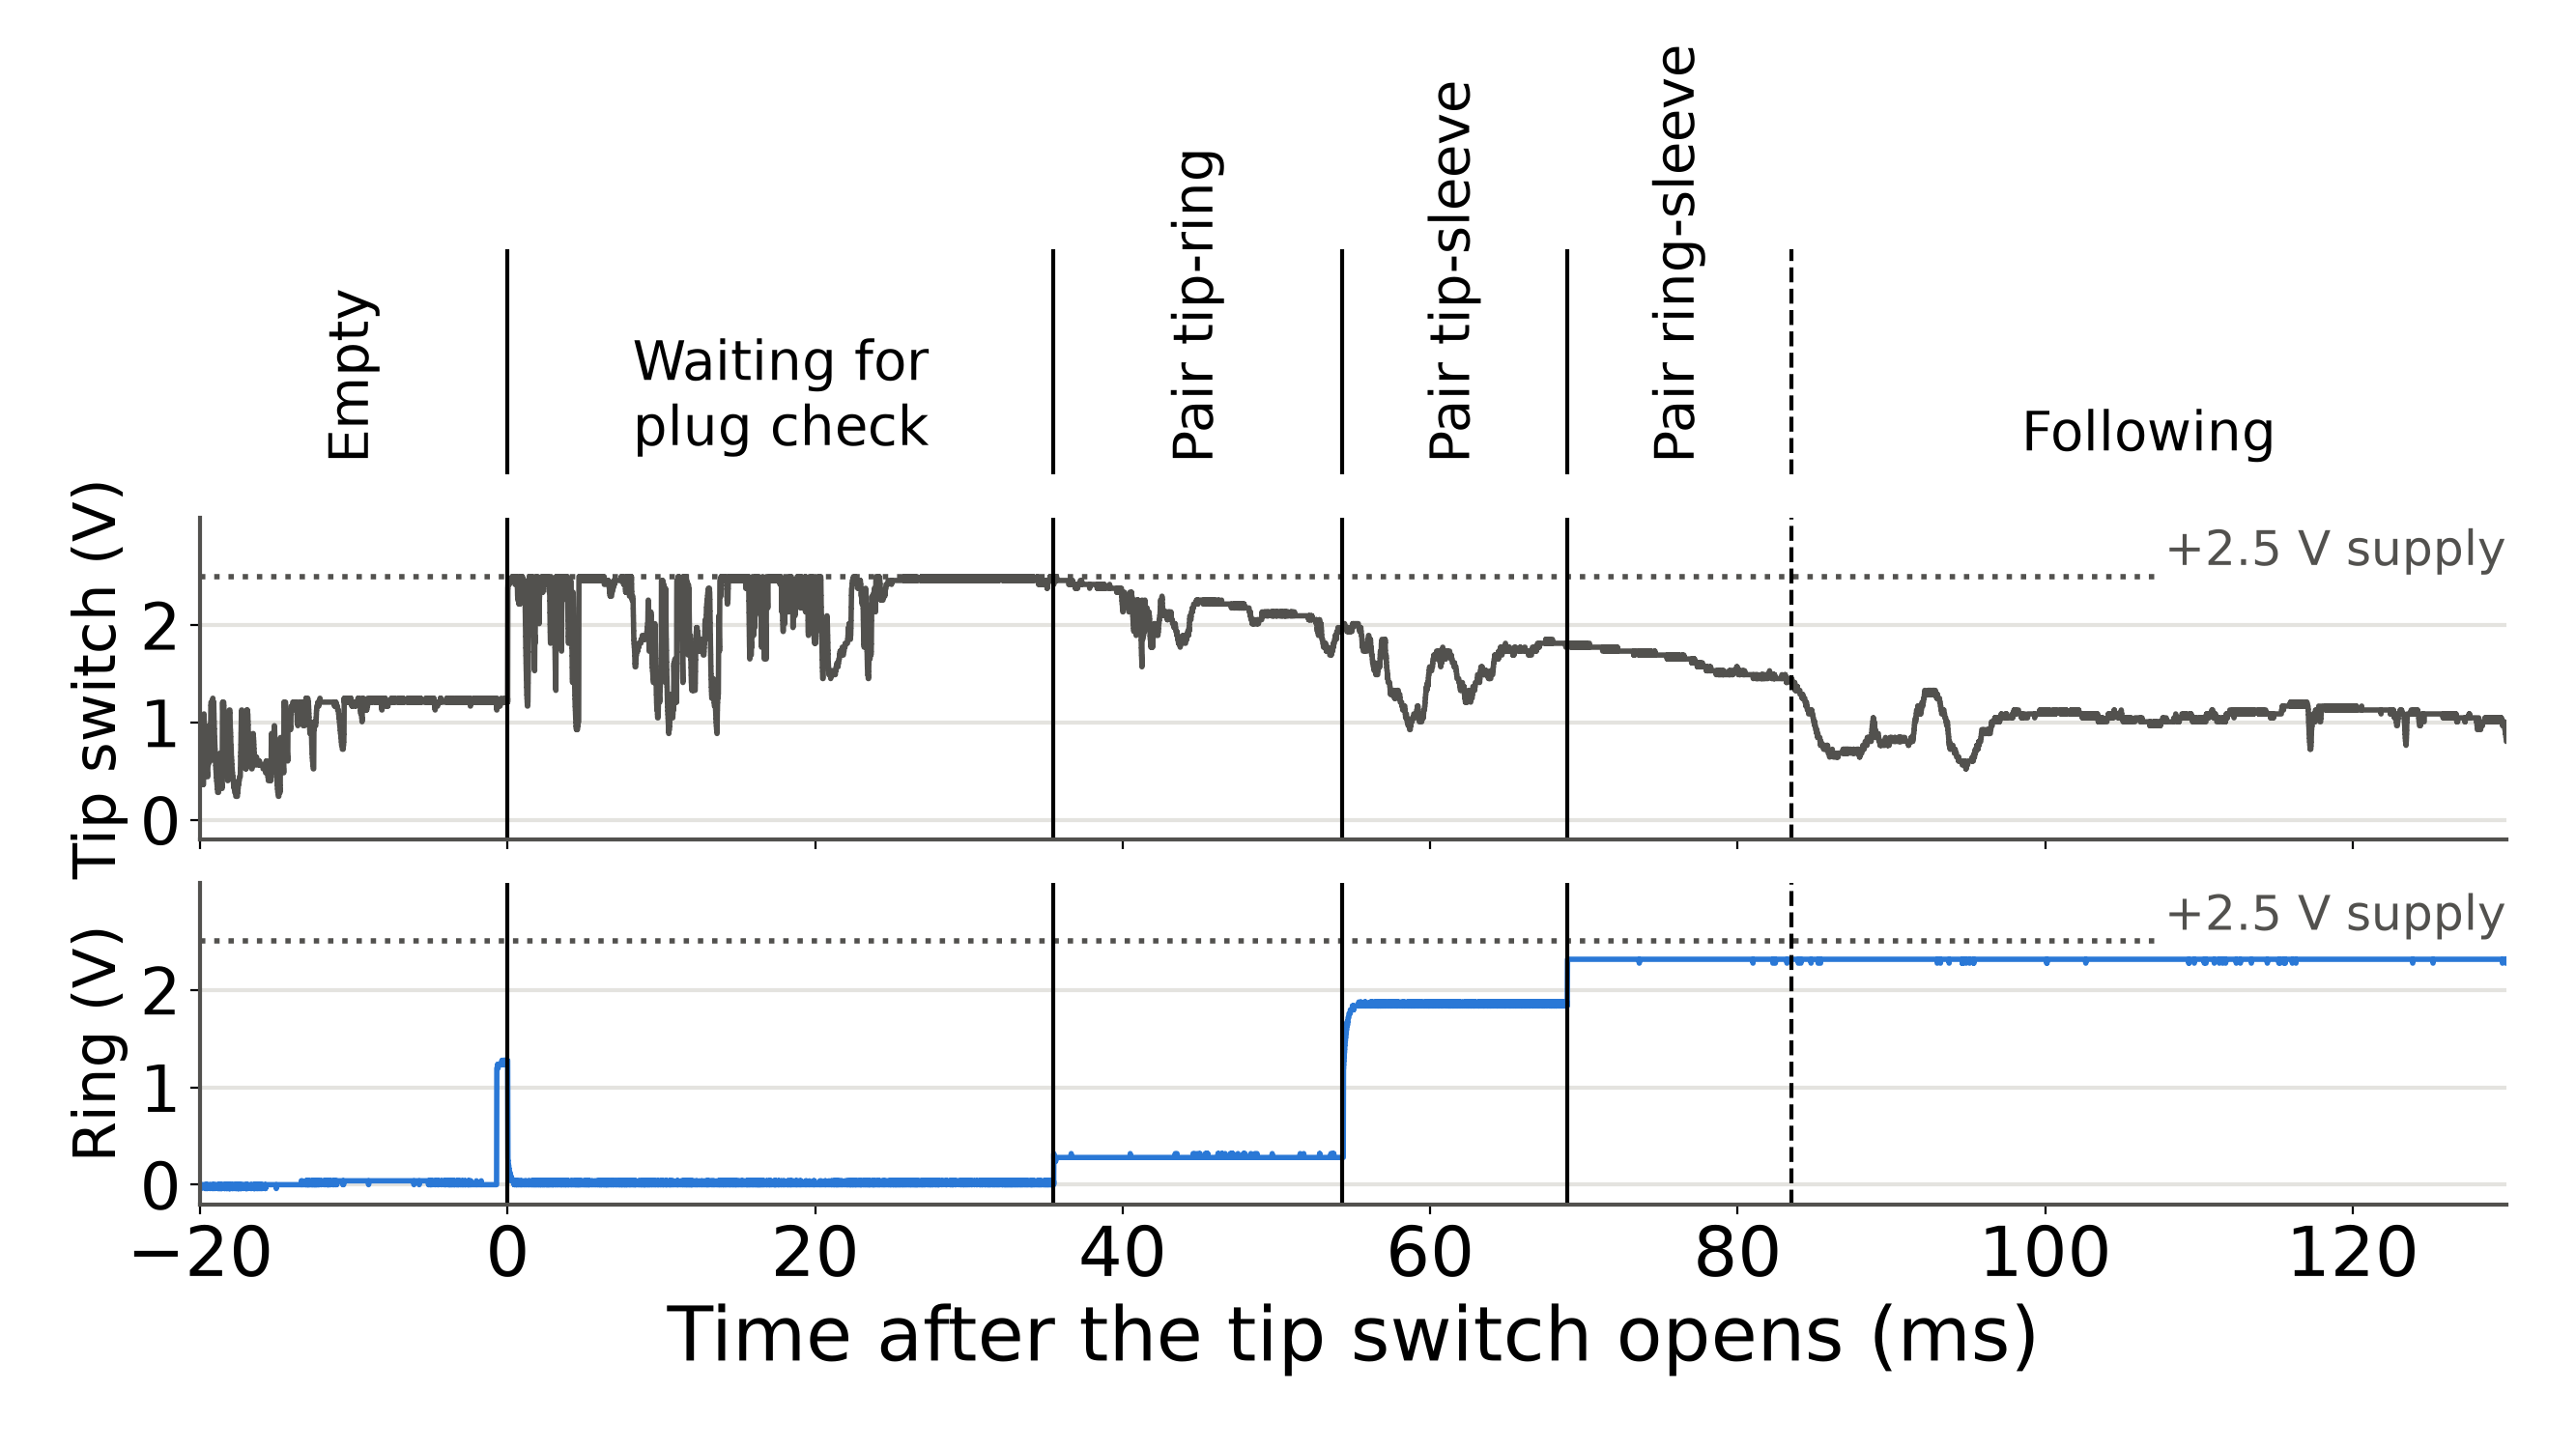
\includegraphics[width=\linewidth]{05-results/figures/plug-in-fresh-rails}
    \caption{Plug-In with Fresh Rails}
    \label{fig:plug-in-fresh}
  \end{subfigure}%
  \hfill%
  \begin{subfigure}[b]{0.49\linewidth}
    \centering
    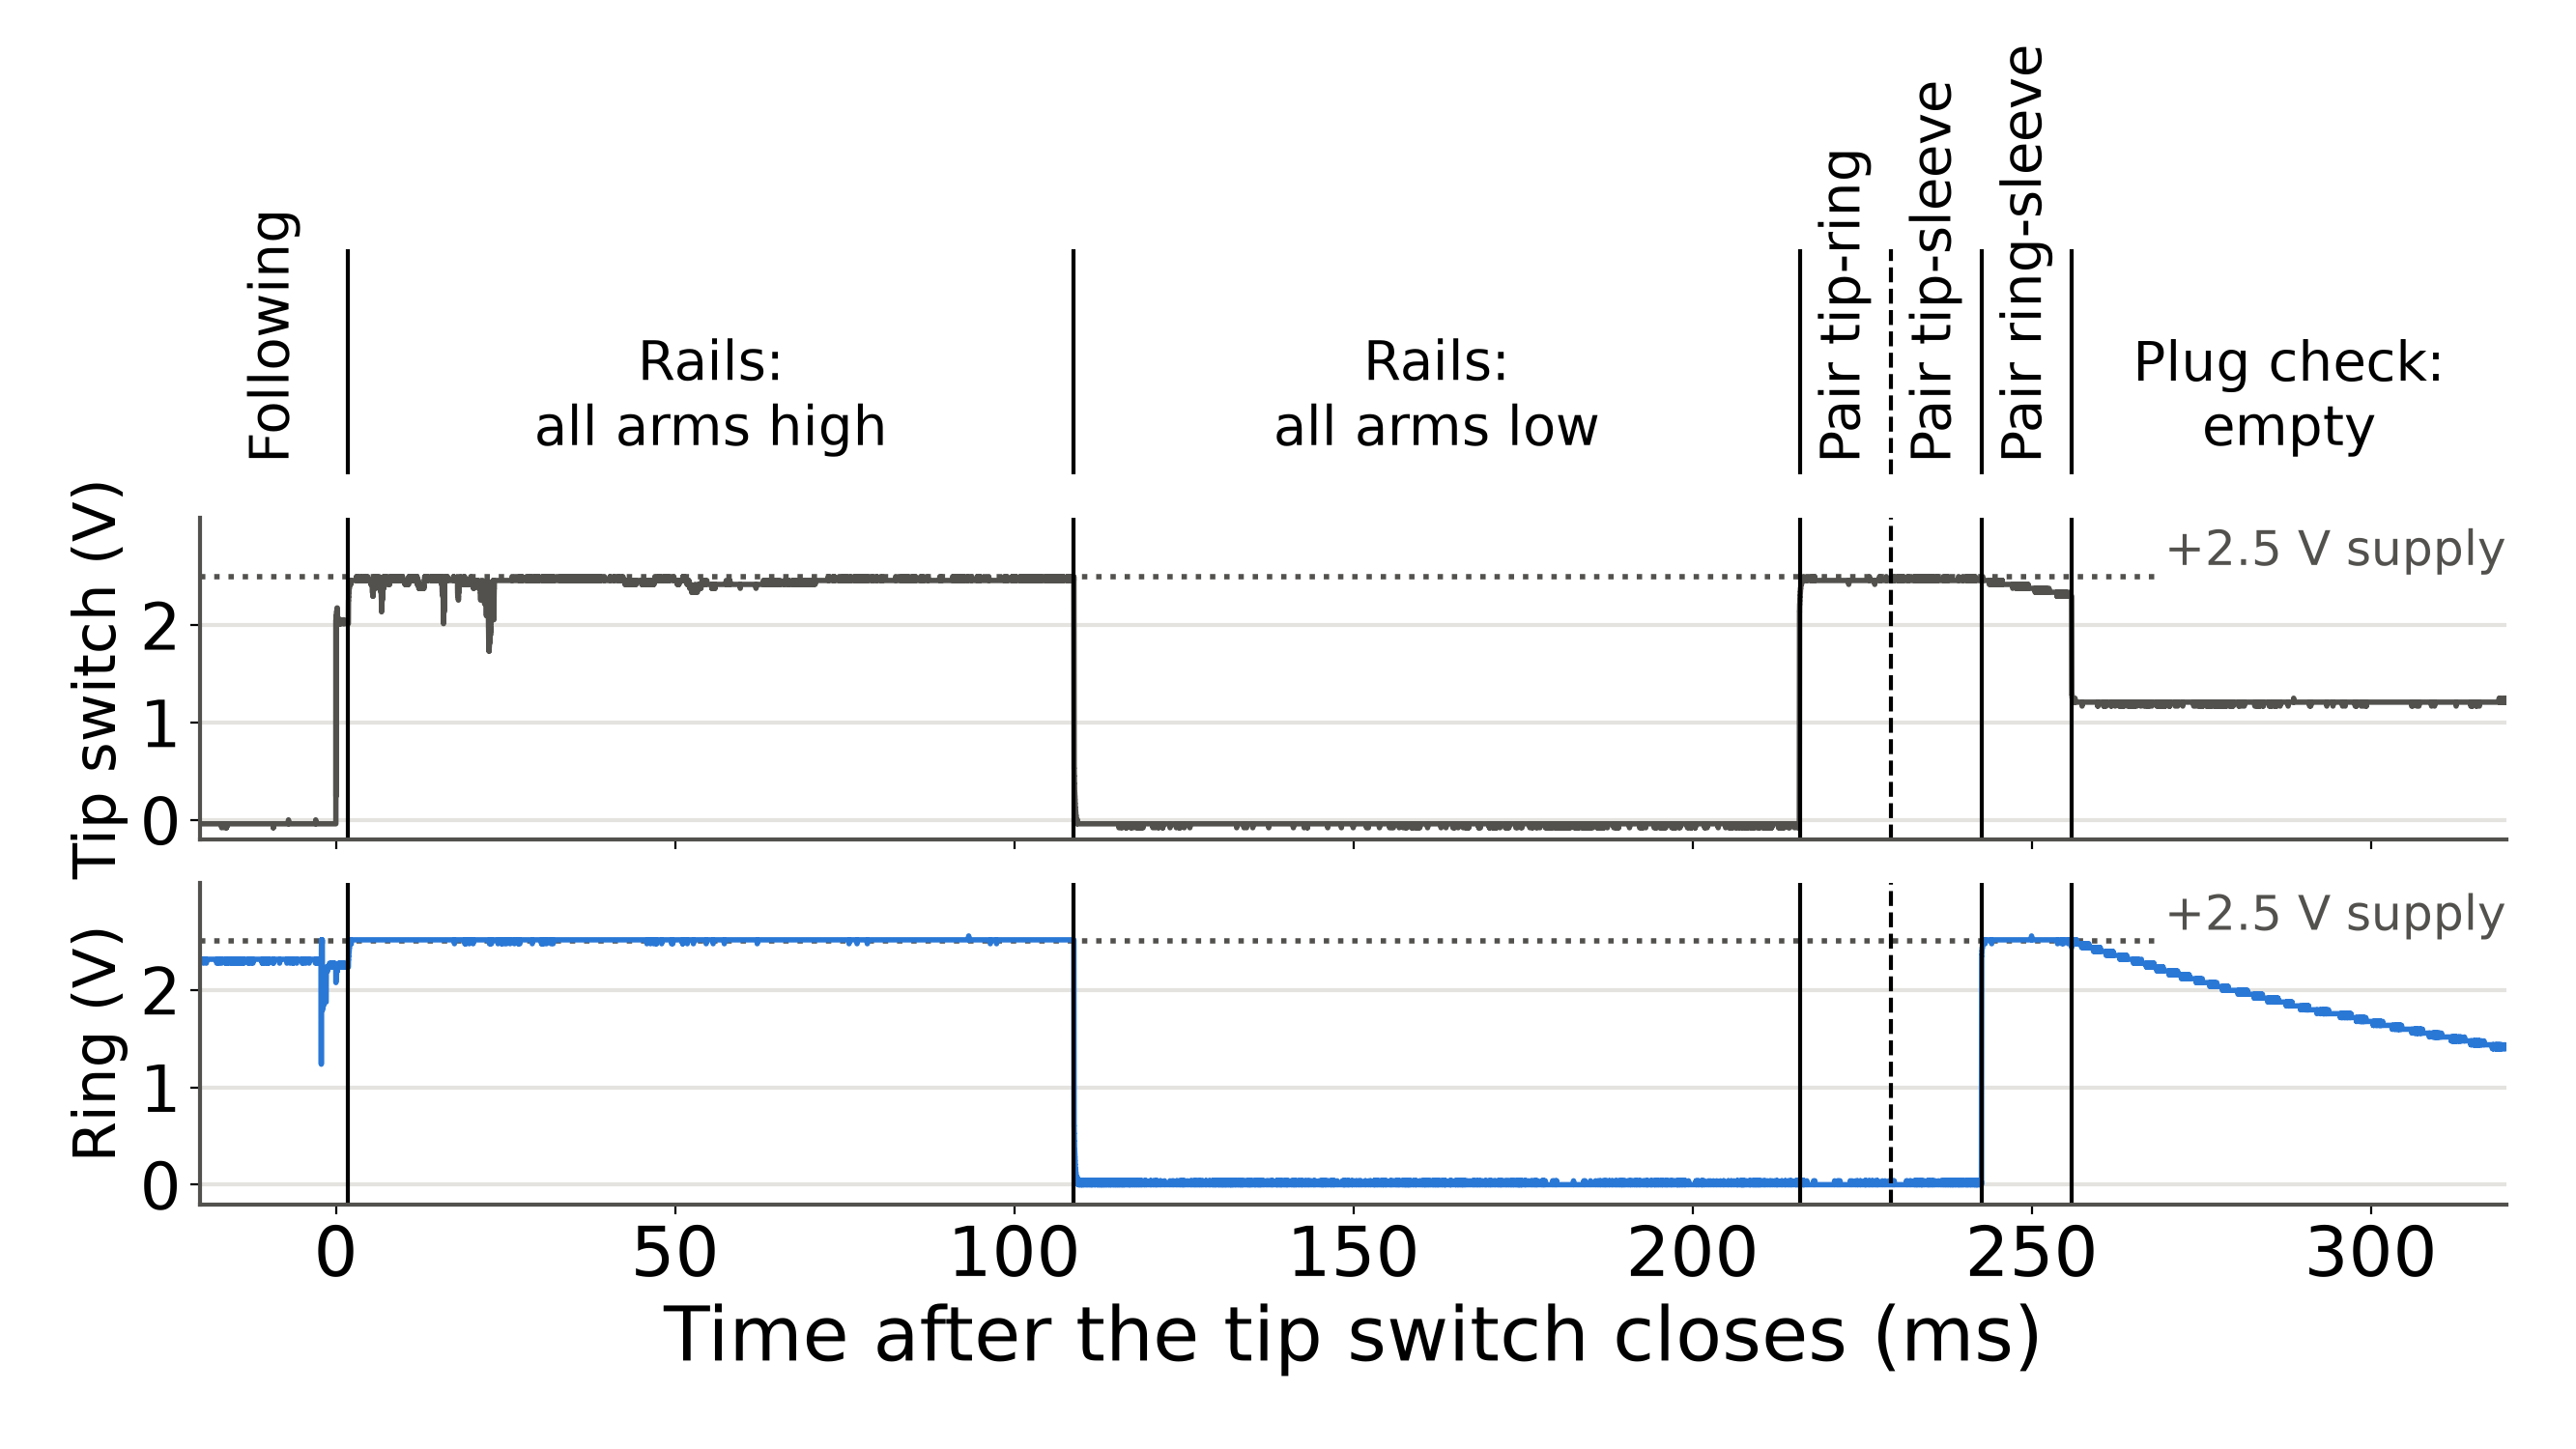
\includegraphics[width=\linewidth]{05-results/figures/unplug}
    \caption{Unplug}
    \label{fig:unplug}
  \end{subfigure}
  \titledcaption{Plug-In and Unplug}{\scaffoldinline{Same setup as \cref{fig:plug-in-refresh}; captures \code{plugin5.csv} and \code{unplug1.csv}.}}
  \label{fig:plug-unplug}
\end{figure}

\begin{figure}[htbp]
  \centering
  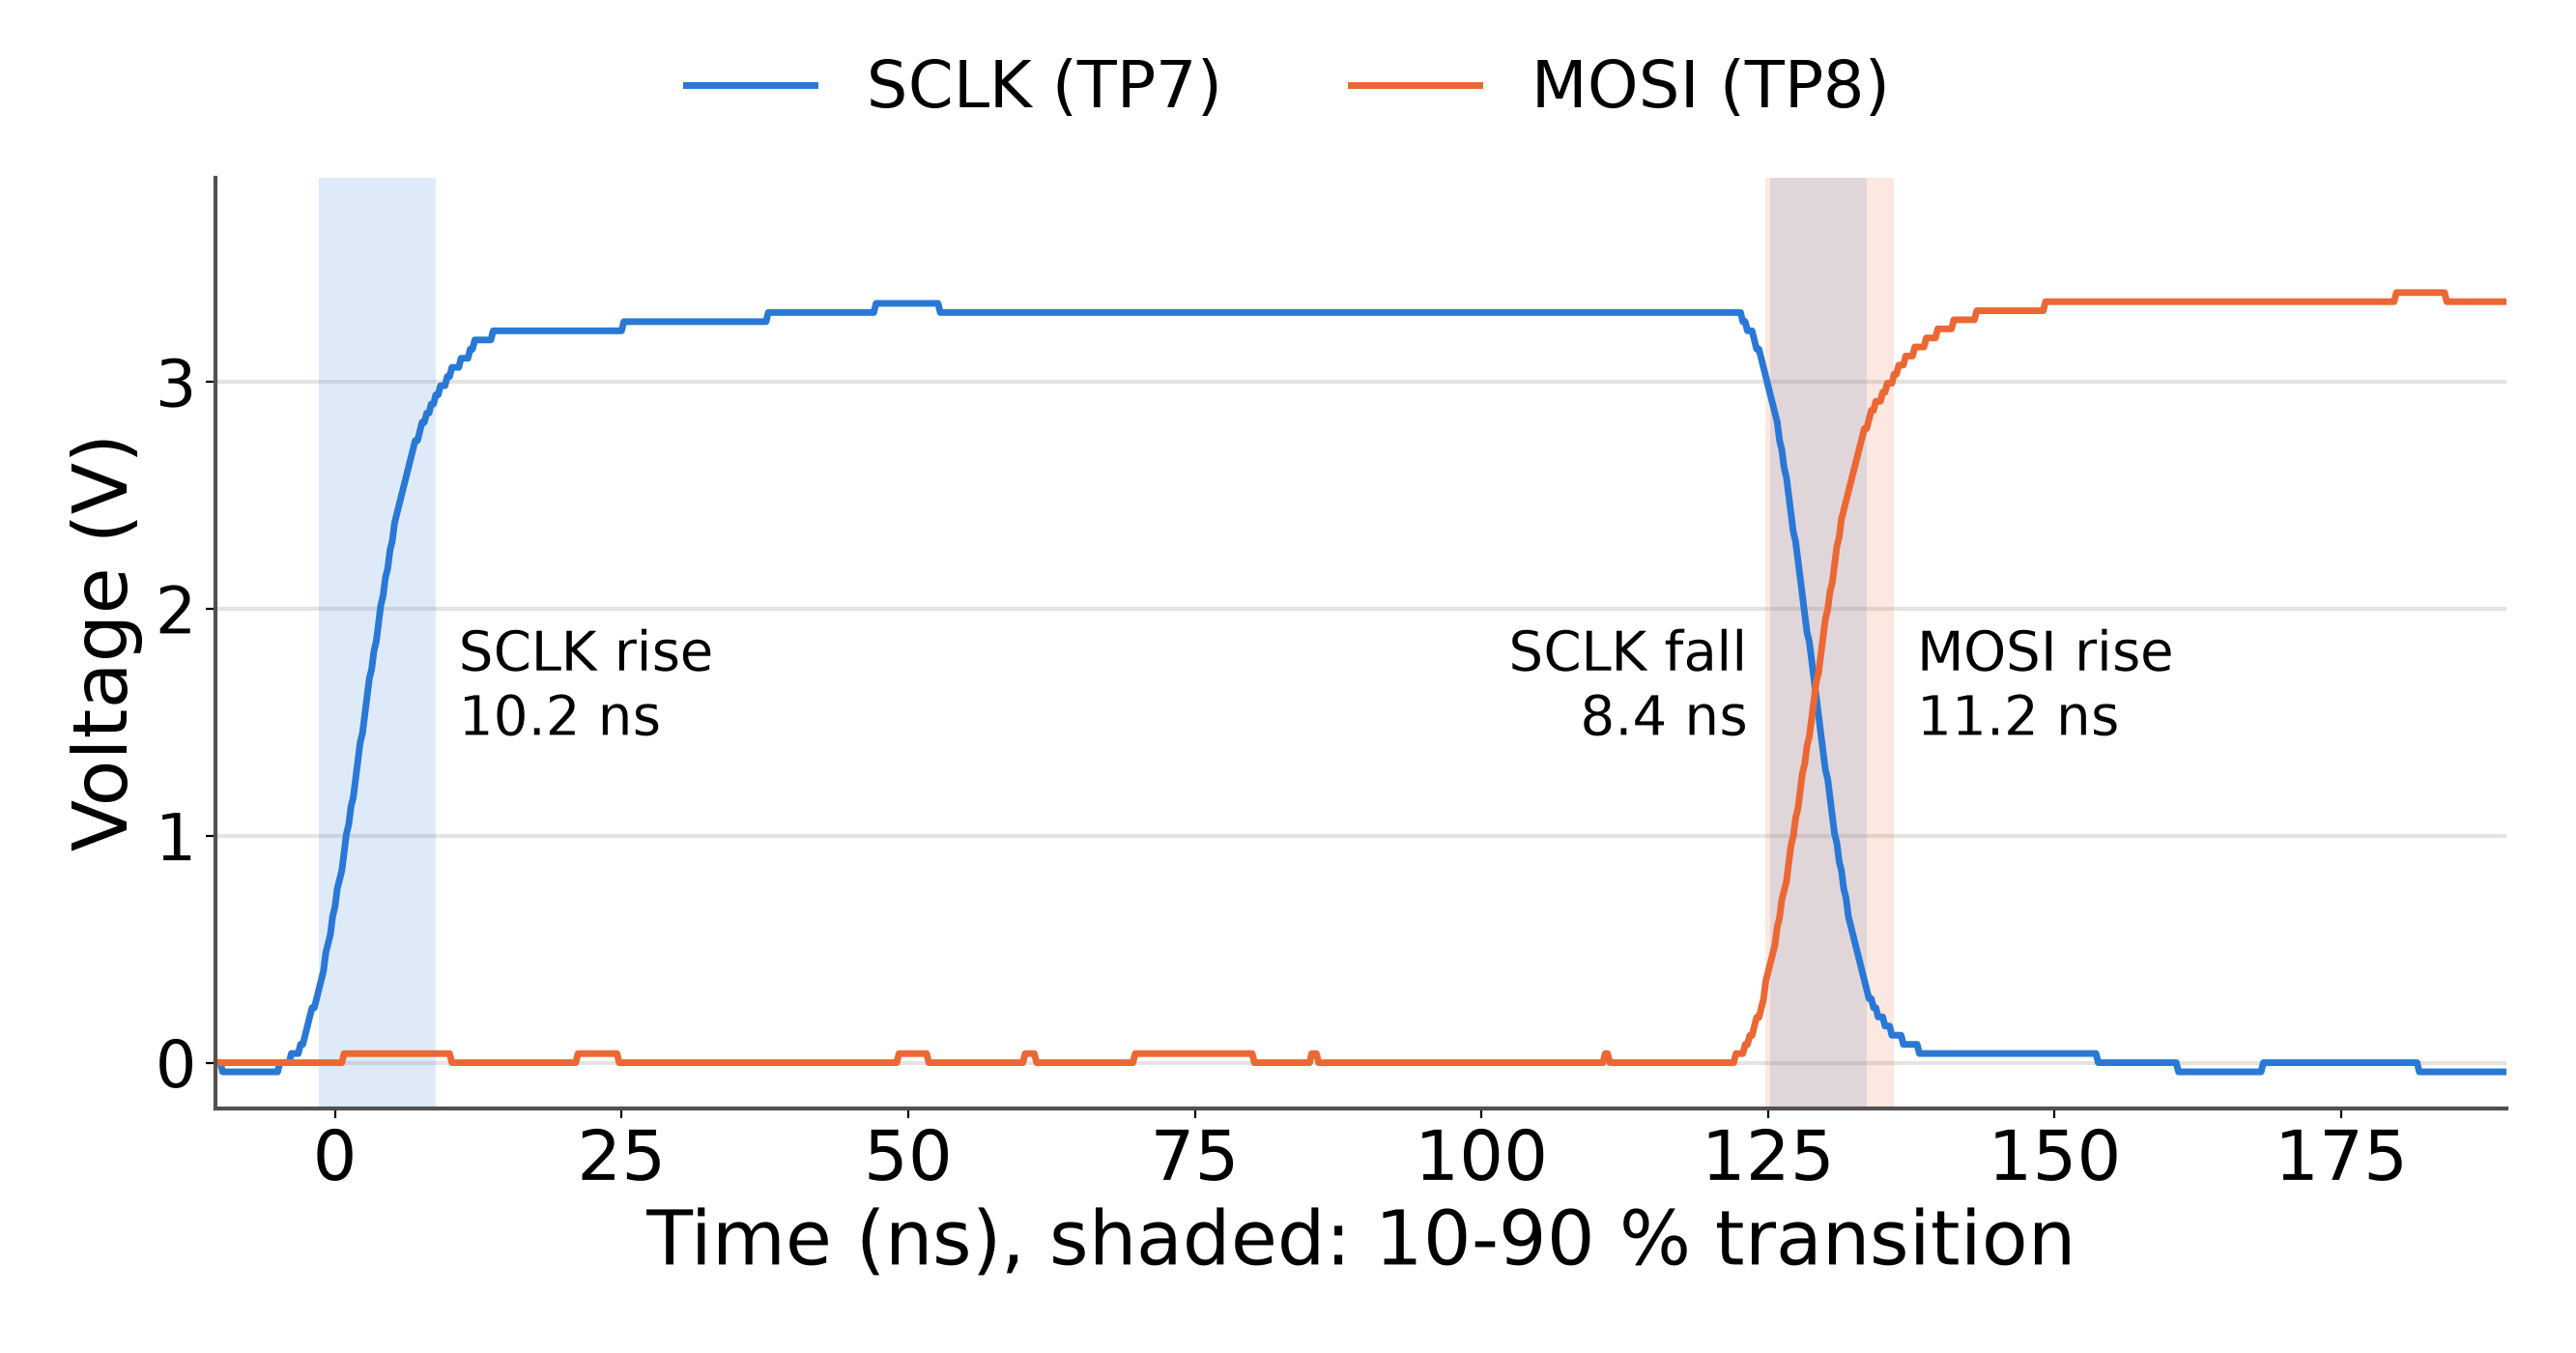
\includegraphics[width=0.7\linewidth]{05-results/figures/spi-edges}
  \titledcaption{SPI Edges}{\scaffoldinline{10X probes, SCLK at TP7, MOSI at TP8, averaged capture; shaded: 10 to \qty{90}{\percent} transitions.}}
  \label{fig:spi-edges}
\end{figure}
